% Déclaration du type de document (report, book, paper, etc...)
\documentclass[a4paper, 12pt]{paper} 
 
% Package pour avoir Latex en français
\usepackage[utf8]{inputenc}
\usepackage[T1]{fontenc}
 
% Quelques packages utiles
\usepackage{listings} % Pour afficher des listings de programmes
\usepackage{graphicx} % Pour afficher des figures
\usepackage{amsthm}   % Pour créer des théorèmes et des définitions
\usepackage{amsmath}
\usepackage{microtype} % Optical margins FTW
\usepackage{url}
\usepackage{booktabs} % Allows the use of \toprule, \midrule and \bottomrule in tables for horizontal lines
\usepackage[per-mode=symbol]{siunitx}
\usepackage{floatrow}
\usepackage{caption}
\usepackage{subcaption}
\usepackage{fullpage}
\usepackage{lipsum}



\author{Loïc Amez-Droz \and Florian Reinhard}
\title{Multimode Fibre}

% Début du document
\begin{document}
\begin{titlepage}
\begin{center}
    \textsc{\LARGE École Polytechnique Fédérale de~Lausanne}\\[1.5cm] 
    {\huge \bfseries Optical Engineering: Multimode Fibre}\\[0.4cm] 
    \begin{tabular}{|p{5cm}|p{4cm}|}
        \hline
        Group & C-XX \\ \hline
        Students & Loïc \textsc{Amez-Droz} \newline Florian \textsc{Reinhard} \\ \hline
        Date of lecture & 13.03.2015 \\ \hline
        Date of final report return & 20.03.2015 \\ \hline
    \end{tabular}
\end{center}


\begin{abstract}
    \lipsum[3]
\end{abstract}
 
\vfill
\end{titlepage}

\section{Procedures and results}
\subsection{Evaluation of the numerical aperture with skewed rays}
\subsection{Measurement of the numerical aperture}
% distance error: 0.01mm
\subsection{Injection for different sources}

\begin{figure}[H]
    \centering
    \begin{subfigure}[b]{0.30\textwidth}
        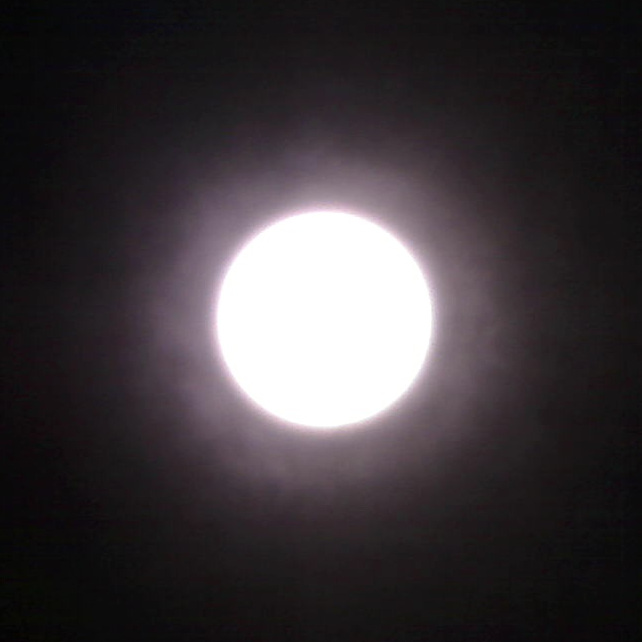
\includegraphics[width=\textwidth]{img/halogen-injection.jpg}
        \caption{Halogen.}
    \end{subfigure}
    \begin{subfigure}[b]{0.30\textwidth}
        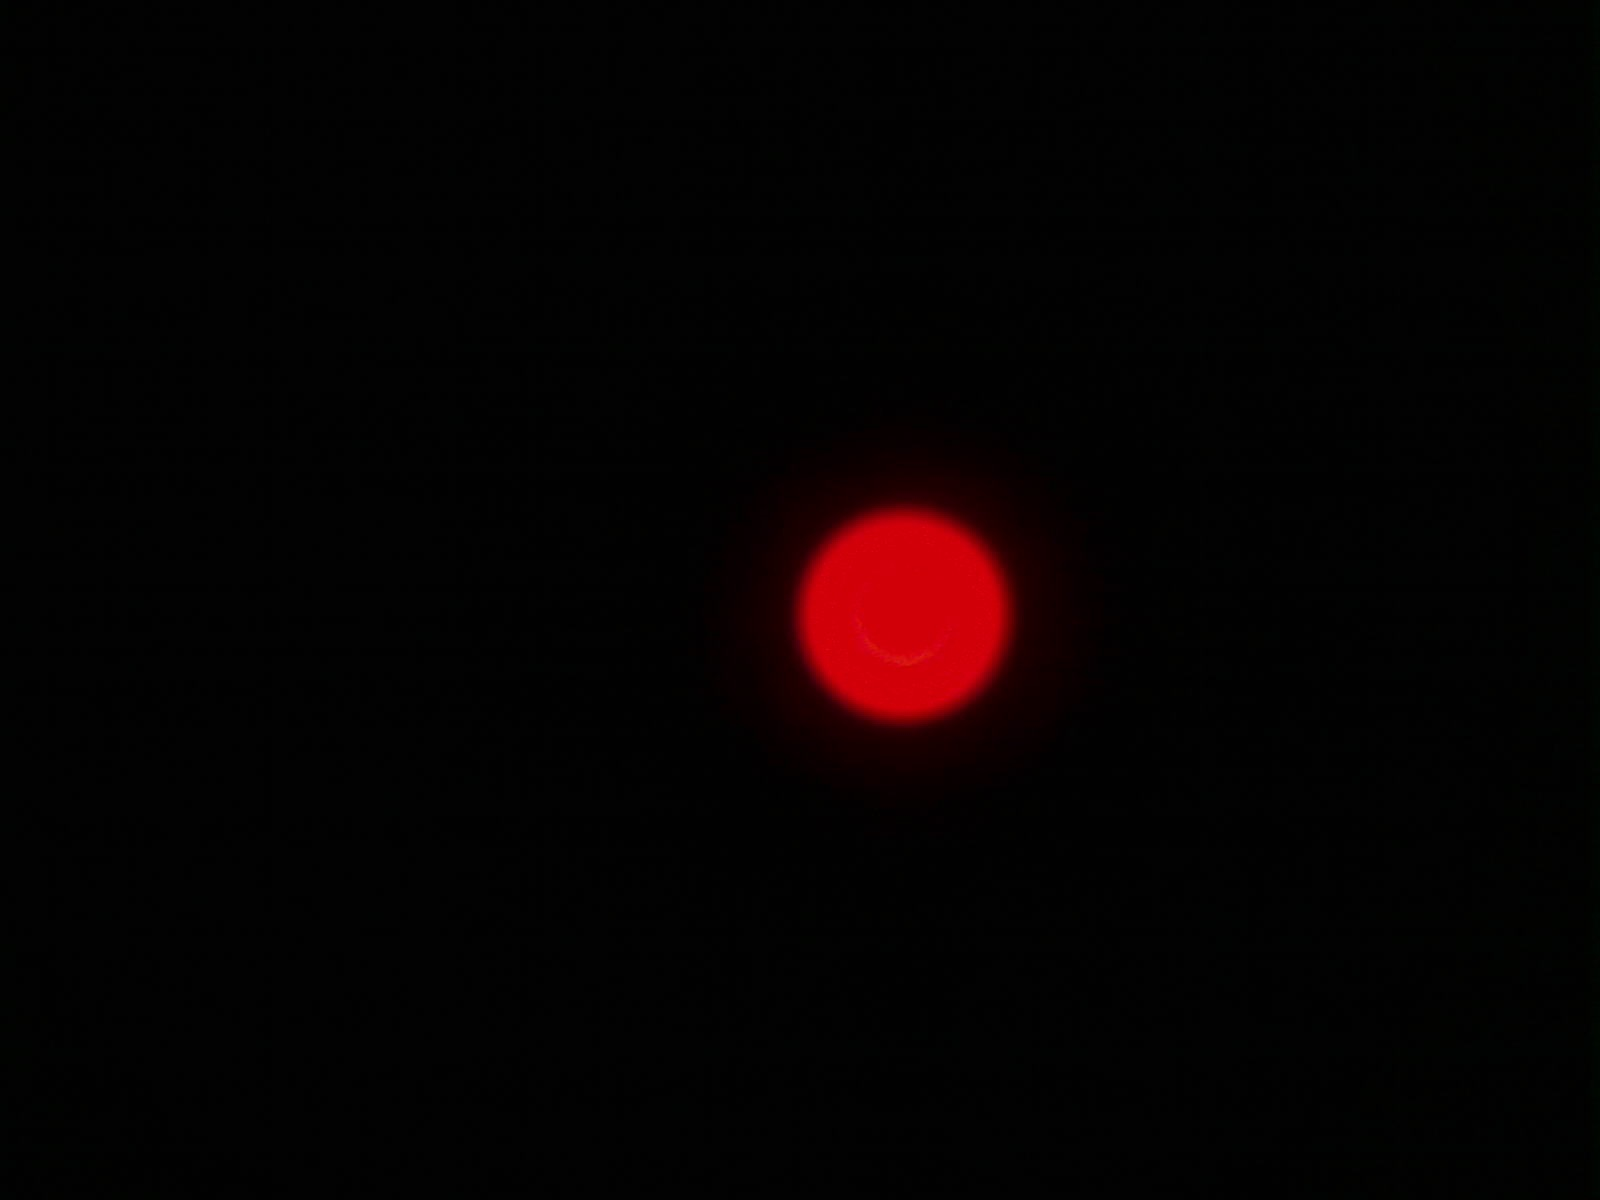
\includegraphics[width=\textwidth]{img/efficiency-45mm.jpg}
        \caption{LED.}
    \end{subfigure}
    \begin{subfigure}[b]{0.30\textwidth}
        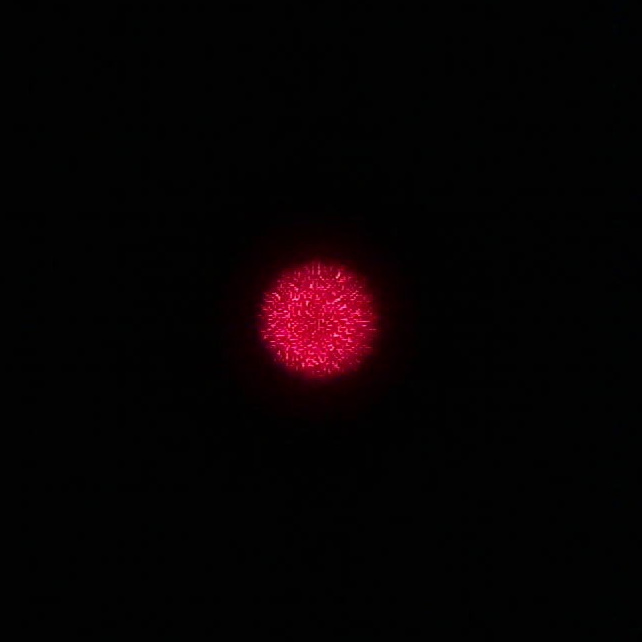
\includegraphics[width=\textwidth]{img/laser-injection.jpg}
        \caption{Laser.}
    \end{subfigure}
    \caption{Injection of different sources.}
\label{fig:sources_injection}


\end{figure}
\subsection{Measurement of relative injection efficiency}

\section{Discussion and conclusions}
\lipsum[6]
\end{document}
